\gls{wrtc} deviates from traditional enterprise collaboration systems by opening up communications from every web application instead of controlled software pieces. So how do we make the open web interoperate with the closed enterprise world. There are two ways of going about this problem. We can either choose to redo the whole existing architecture of the enterprise collaboration system putting \gls{wrtc} technology in the center and upgrade all the existing infrastructure to support \gls{wrtc}, but this is an expensive solution, especially since the \gls{ietf} has not yet finished deciding upon which protocols and codecs to be used. Therefore, the best option is to extend current architecture with \gls{wrtc} capabilities. To do this we have to create a gateway between the underlying technologies of \gls{wrtc} specified as \gls{rtcweb} and existing enterprise infrastructure. The aim when creating a gateway between the two systems is to re-use as much as possible of existing architecture.

\section{Requirements and problems}
There are basically three planes we have to make interoperate: the signaling plane, the media plane, and the IP addressing plane. 
By signaling we mean the offer/answer exchange. The media plane is the transportation of the media, and the IP addressing plane is basically how we connect to each other.

\begin{figure}[here]
\centerline{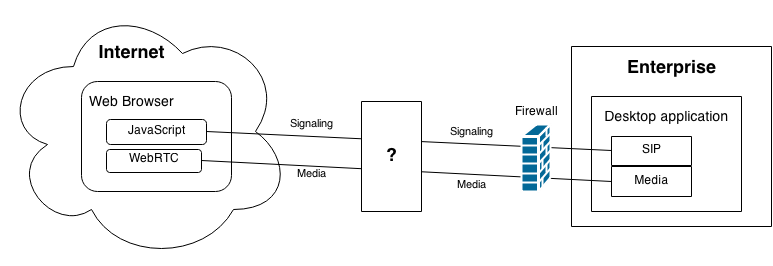
\includegraphics[scale=0.5]{gateway-layers.png}}
\caption{WebRTC-Enterprise interworking}
\label{fig:gateway-layers}
\end{figure}

\subsection{Signaling}
\gls{wrtc} does not define any standard way of doing signaling, but we do have to implement it and get it working with typical enterprise ways of doing this. In order to get a session going, the peers should only have the need to exchange four things for establishing a secure connection in addition to information about the media:

\begin{itemize}
\item{An ICE username}
\item{An ICE password}
\item{A list of possible ICE candidates}
\item{A DTLS fingerprint}
\end{itemize}

The current \gls{wrtc} specification says to exchange this information with the browser API in \gls{sdp} format. \gls{sdp} is an old format used in the \gls{voip} world, therefore the re-use of \gls{sdp} is supposed to save time, but the anatomy of an \gls{sdp} is complex and constantly changing because the \gls{ietf} are coming up with new stuff to include. All the information has to be excactly right or it will be rejected by the browser. It is highly unlikely that the current specification of \gls{sdp} will work with any older implementation found in any enterprise communication system.

Another thing is that \gls{wrtc} has to do signaling running over \gls{http}, while the standard in an enterprise system is to use \gls{sdp} with \gls{sip} or some other proprietary way over \gls{tcp} or \gls{udp}.

We need to come up with some way of manipulating the \gls{sdp} and possibly use a \gls{sip} stack developed in Javascript running in the client.

\subsection{Media}
In the \gls{wrtc} world the media plain is designed to avoid having to relay media streams. The goal is to have pure peer-to-peer connections, while in the enterprise world it is common to have full control over the media plane and in most cases use some kind of media server. Also the \gls{wrtc} specification says that support for \gls{ice} and \gls{srtp}-\gls{dtls} are mandatory. Encryption is hardly ever used in the enterprise world, so this is another challenge. If encryption is used, it is more common to use \gls{srtp}-\gls{sdes} with the keys being handled on the signaling plane, rather than in media plane that is the case with \gls{dtls}.

\gls{wrtc} uses one-way media streams, while an enterprise system usually expects to receive bi-directional streams. This can be fixed by multiplexing the streams, so we can have multiple streams running over the same network port.

The biggest issues here is probably which codecs we need to implement. The \gls{ietf} has landed on two default audio codecs, but has not decided on which video codec to use yet. The most typical enterprise video code used is H.264. Right now the \gls{ietf} are deciding between VP8 and H.264, so currently we have to support both and do server side transcoding between them.

\subsection{IP addressing}
In the enterprise world a \gls{sbc} is commonly used to control incoming media traffic. In \gls{wrtc} one uses \gls{ice} browser-to-browser to cross firewalls. We have to handle both exchanging of \gls{ice} candidates and bypassing the enterprise firewall. This is a bigger topic that we will go more deeply into in the next chapter.

\section{Summary}
The first iteration of \gls{rtcweb} is still under development, and not all protocols and codecs have been decided yet. It is theoretically possible to create a gateway and it has been done before under closed doors. Some of the biggest issues are how to handle the signaling, translating the media, and crossing the enterprise firewall. In the next chapter we will further look into how to traverse the enterprise firewall before we finally introduce a solution to the problem.
